\chapter{AdS/CFT in the large-\texorpdfstring{$N$}{N} limit: an algebraic formulation}

Chapters~2--5 developed their tools on their own terms. They used nothing more exotic than qubits, matrix
algebras, and (in Chapter~4) an ordinary free quantum field. This chapter applies all of those tools (the type
classification, the GNS construction, modular theory, and the crossed product) to the physical system these notes
are aiming at. That system is the AdS/CFT correspondence, in the limit $N\to\infty$, or equivalently $G_N\to0$,
where bulk spacetime is supposed to emerge.

\section{General description}

\subsection*{The dictionary, restated precisely}

AdS/CFT is a conjecture. It says that quantum gravity on $(d{+}1)$-dimensional anti-de~Sitter space (AdS) is
completely equivalent to an ordinary conformal field theory (CFT), without gravity, living on the
$d$-dimensional boundary of that space. The standard example is type IIB string theory on
$\text{AdS}_5\times S^5$, which is dual to $\mathcal N=4$ super-Yang-Mills theory with gauge group $SU(N)$.

The core entries of the dictionary are these.
\begin{itemize}
\item The two theories share the same Hilbert space, $\HH_{\text{bulk}}=\HH_{\text{CFT}}\equiv\HH$.
\item The classical-gravity limit $G_N\to0$ is the same as the large-$N$ limit of the boundary gauge theory.
\item The limit $\alpha'\to0$ is the same as the limit of infinite 't~Hooft coupling, $\lambda\to\infty$, in the
boundary theory. Here $\alpha'$ sets the string length, so $\alpha'\to0$ switches off stringy corrections.
\item Elementary bulk fields correspond to \textbf{single-trace operators}. These are boundary operators built as
a single trace over color indices, $\Tr(\cdots)$.
\item A classical bulk geometry $\phi_c$ corresponds to a specific boundary state $\ket\Psi$, called a
\textbf{semiclassical state}.
\end{itemize}

The precise map from bulk fields to boundary operators is the \textbf{extrapolate dictionary}:
\begin{equation}
O(x) = \lim_{r\to\infty} r^\Delta\,\phi(r,x) .
\label{eq:ads-extrapolate}
\end{equation}
In words: take a bulk field $\phi$ and evaluate it at radial coordinate $r$ and boundary point $x$. Multiply by
$r^\Delta$, where $\Delta$ is the conformal dimension of the operator, a number fixed by the mass of the field.
Then send $r\to\infty$, which moves the point out to the AdS boundary. What survives this limit is the
corresponding boundary operator $O(x)$.

This equation is not just a convenient definition. In some holographic theories an independent definition of
$O(x)$ already exists, such as $\Tr(\cdots)$ in super-Yang-Mills. There, \eqref{eq:ads-extrapolate} is a derived
fact. In more general holographic systems no such independent definition is available. There,
\eqref{eq:ads-extrapolate} \emph{is} taken as the definition of what counts as a single-trace operator.

A semiclassical state $\ket\Psi$ is one with a well-defined $N\to\infty$ limit. This means it can be built as
the limit of a sequence of states $\{\ket{\Psi_N}\}$, one for each finite-$N$ theory. This chapter works out two
examples. The first is the vacuum $\ket\Omega$, dual to empty AdS. The second is the thermofield double
$\ket{\Psi_\beta}$, which at high enough temperature is dual to an eternal black hole. A third example is a
single-sided black hole formed by collapse. It is generally harder to write down explicitly.

\subsection*{Building the boundary operator algebra with GNS, and why it can be bigger than expected}

Here the tools of Chapters~2 and~4 are used directly. Say that an operator $A$ has a well-defined large-$N$
limit in the state $\ket\Psi$ if two things hold. First, $A$ is the limit of some sequence of finite-$N$
operators $\{A_N\}$, with corresponding states $\{\ket{\Psi_N}\}$. Second, the expectation values converge to
something finite:
\[
\lim_{N\to\infty}\braket{\Psi_N|A_N|\Psi_N}<\infty .
\]
This is the same kind of finite-energy restriction met for the infinite chain of Bell pairs in Chapters~1
and~2, now applied to a real gauge theory. Call the collection of all such operators $\Alg_\Psi$. One subset is
present for every semiclassical state:
\[
\Sscr \equiv \text{the } *\text{-algebra generated by single-trace operators} \subseteq \Alg_\Psi .
\]
The inclusion need not be an equality. The set $\Alg_\Psi$ may contain \emph{more} operators than those built
from single-trace operators, and which extra operators survive can depend on the state $\Psi$. This point is
easy to skip on a first reading. But the fact that the inclusion can be strict turns out to be exactly what
allows a description of a black-hole \emph{interior}. This is discussed in the section on general black holes
below.

Assume that $\Alg_\Psi$ is closed under products, so it is a $*$-algebra. Assume also that it is completed in
the norm it inherits, so it is a $C^*$-algebra, exactly the kind of object studied in Chapter~2. Then
expectation values in $\ket\Psi$ define a state $\omega_\Psi$ on $\Alg_\Psi$. The GNS construction of Chapter~2
applies directly. It gives a GNS Hilbert space $\HH_\Psi^{\text{GNS}}$ built from $(\Alg_\Psi,\omega_\Psi)$,
together with a representation $\pi_\Psi(\Alg_\Psi)$. This Hilbert space is, quite literally, ``the space of
small excitations around $\ket\Psi$.'' It is the same construction that Chapter~2 carried out by hand on qubits.

Suppose the bulk geometry dual to $\Psi$ is smooth and $\Psi$ is pure. Then $\omega_\Psi$ is expected to be a
pure state on $\Alg_\Psi$. Chapter~2 showed that a pure state gives an irreducible GNS representation. So
\begin{equation}
B(\HH_\Psi^{\text{GNS}})=\pi_\Psi(\Alg_\Psi)'' .
\label{eq:ads-irreducible}
\end{equation}
This can fail if the dual geometry has a singularity that can be reached on some Cauchy slice. We return to
this in the discussion of firewalls later in this chapter. Write
\[
Y\equiv(\pi_\Psi(\Sscr))'', \qquad Y_O\equiv(\pi_\Psi(\Sscr_O))''
\]
for the von Neumann algebra generated by single-trace operators alone, and for its restriction to a boundary
region $O$. The algebra $Y$ may be strictly smaller than $\pi_\Psi(\Alg_\Psi)''$.

\subsection*{Matching this to an ordinary bulk Fock space}

On the gravity side, expand every bulk field around its classical background:
$\phi=\phi_c+\kappa\delta\phi$, with $\kappa=\sqrt{8\pi G_N}$. This gives an action
$S[\phi_c]+S_2[\delta\phi]+S_{\text{int}}[\delta\phi]$, with $S_{\text{int}}=\kappa S_3+\kappa^2S_4+\cdots$. At
leading order, $\kappa\to0$, only the quadratic piece $S_2$ survives. It describes an ordinary free quantum field
$\delta\phi$ on the fixed background $\phi_c$. Quantizing it in the standard way, with some vacuum
$\ket0_{\phi_c}$, gives a Fock space $\HH_\Psi^{\text{Fock}}$.

We now have two Hilbert spaces. One is built from the boundary algebra by GNS. The other is built from the bulk
field theory by ordinary quantization. For the AdS/CFT duality to hold, they must agree:
\begin{equation}
\HH_\Psi^{\text{Fock}} = \HH_\Psi^{\text{GNS}} .
\label{eq:ads-fock-gns}
\end{equation}
This requires the GNS representation to have exactly the structure of a Fock space. In other words, the
boundary theory must be Gaussian at large $N$: all correlators must factorize into products of two-point
functions. This property is called ``large-$N$ factorization.'' It follows from 't~Hooft's planar scaling, as
the following sketch shows.

\begin{keyresult}[: Sketch of the large-$N$ generalized free field and its CCR algebra]
\textbf{Goal:} Explain why, in a large-$N$ $SU(N)$ gauge theory with fixed 't~Hooft coupling $\lambda = g_{YM}^2 N$:
\begin{enumerate}
\item Connected correlators of $n$ single-trace operators scale as $\braket{\mathcal{O}_1 \cdots \mathcal{O}_n}_{\text{conn}} \sim N^{2-n}$.
\item Commutators of single-trace operators become $c$-numbers: $[\mathcal{O}_A, \mathcal{O}_B] = c_{AB}\id + O(1/N)$.
\item The resulting boundary algebra is a CCR algebra, whose GNS space is a free Fock space $\HH_\Psi^{\text{Fock}}$.
\end{enumerate}
This is a standard diagrammatic argument, not a rigorous proof.

\textbf{Derivation sketch:}
\begin{enumerate}[leftmargin=*]
\item \textbf{The 't~Hooft topological expansion.}
Consider an adjoint matrix field theory with action $S = \frac{N}{\lambda}\int d^d x \Tr\big[\frac{1}{2}(\partial\Phi)^2 + V(\Phi)\big]$. So the propagator carries a factor $g_{YM}^2=\lambda/N$ and each interaction vertex a factor $1/g_{YM}^2=N/\lambda$. In 't~Hooft's double-line notation, a vacuum Feynman graph with $V$ vertices, $E$ edges (propagators), and $F$ closed index loops scales as
\begin{align}
(g_{YM}^2)^{E-V} N^F
&\eqstep{1} \lambda^{E-V} N^{V - E + F}
\ \eqstep{2}\ \lambda^{E-V} N^\chi
\ \eqstep{3}\ \lambda^{E-V} N^{2 - 2g} . \notag
\end{align}
\stepwhy{1}{substitute $g_{YM}^2=\lambda/N$, so $(g_{YM}^2)^{E-V}=\lambda^{E-V}N^{-(E-V)}$.}\quad
\stepwhy{2}{$\chi\equiv V-E+F$ is the Euler characteristic of the surface on which the double-line graph can be
drawn.}\quad
\stepwhy{3}{for a closed orientable surface of genus $g$, $\chi=2-2g$.}

The leading diagrams are planar, with the topology of a sphere ($g = 0$, $\chi = 2$). They contribute at order $N^2$.

\item \textbf{Scaling of connected correlators.}
Define the single-trace operators, with their vacuum value subtracted,
\[
\mathcal{O}_i(x) \equiv \Tr\big(\Phi^{k_i}(x)\big) - \Braket{\Tr\big(\Phi^{k_i}(x)\big)} .
\]
Now consider a connected correlator $\braket{\mathcal{O}_1(x_1) \cdots \mathcal{O}_n(x_n)}_{\text{conn}}$. Treat each operator insertion as an extra vertex of the graph, so the graph has $V_{\rm int}$ interaction vertices and $n$ insertions. An interaction vertex carries a factor $N/\lambda$ from the action. An insertion carries no such factor. Therefore
\begin{align}
\Big(\frac N\lambda\Big)^{V_{\rm int}}\Big(\frac\lambda N\Big)^{E}N^F
&\eqstep{4} \lambda^{E-V_{\rm int}}\,N^{(V_{\rm int}+n)-E+F}\,N^{-n} \notag\\
&\eqstep{5} \lambda^{E-V_{\rm int}}\,N^{\chi-n}
\ \eqstep{6}\ \lambda^{E-V_{\rm int}}\,N^{2-n} . \notag
\end{align}
\stepwhy{4}{collect the powers of $N$, and add and subtract $n$ in the exponent.}\quad
\stepwhy{5}{counting the insertions as vertices, the Euler characteristic is $\chi=(V_{\rm int}+n)-E+F$.}\quad
\stepwhy{6}{a connected planar graph has $\chi=2$.}

So
\[
\Braket{\mathcal{O}_1(x_1) \cdots \mathcal{O}_n(x_n)}_{\text{conn}} \sim N^{2-n} .
\]
In terms of canonically normalized fields $\varphi=\Phi/g_{YM}$, the same operators are
$\mathcal O_i=(\lambda/N)^{k_i/2}\Tr\varphi^{k_i}$ minus its mean. For $k_i=2$ this is $\lambda\,N^{-1}\Tr\varphi^2$, the normalization used in the worked example later in this chapter. The leading powers of $N$ are:
\begin{itemize}
\item $n = 2$: $\braket{\mathcal{O}_1 \mathcal{O}_2}_{\text{conn}} \sim N^0 = O(1)$. The two-point function is finite and nonzero.
\item $n = 3$: $\braket{\mathcal{O}_1 \mathcal{O}_2 \mathcal{O}_3}_{\text{conn}} \sim N^{-1} \xrightarrow{N\to\infty} 0$.
\item $n \ge 3$ in general: $\braket{\mathcal{O}_1 \cdots \mathcal{O}_n}_{\text{conn}} \sim N^{2-n} \xrightarrow{N\to\infty} 0$.
\end{itemize}

\item \textbf{Wick's theorem and Gaussian factorization.}
All connected correlators with $n \ge 3$ vanish as $N \to \infty$. By the cumulant expansion, every higher correlation function then splits into a sum of products of two-point functions:
\[
\lim_{N\to\infty} \Braket{\mathcal{O}_1(x_1) \cdots \mathcal{O}_{2m}(x_{2m})} = \sum_{\text{pairings } \pi} \prod_{(i, j) \in \pi} \Braket{\mathcal{O}_i(x_i)\mathcal{O}_j(x_j)} .
\]
Correlators with an odd number of operators vanish. A field with this property is called a \textbf{generalized free field} (GFF).

\item \textbf{Commutators become $c$-numbers.}
Now look at the commutator $[\mathcal{O}_A(x), \mathcal{O}_B(y)]$. Its expectation value is a number,
\[
c_{AB}(x, y) \equiv \Braket{[\mathcal{O}_A(x), \mathcal{O}_B(y)]} \sim O(1) .
\]
The quantum fluctuation of the commutator around this number is controlled by connected four-point functions:
\[
\begin{split}
\Big\| \big([\mathcal{O}_A(x), \mathcal{O}_B(y)] - c_{AB}(x, y)\id\big)\ket\Omega \Big\|^2
&\sim \Braket{\mathcal{O}_A\mathcal{O}_B\mathcal{O}_A\mathcal{O}_B}_{\text{conn}} \\
&\sim N^{2-4} = \frac{1}{N^2} \xrightarrow{N\to\infty} 0 .
\end{split}
\]
The fluctuations vanish as $N \to \infty$, so in the limit the commutator is a $c$-number:
\[
[\mathcal{O}_A(x), \, \mathcal{O}_B(y)] = c_{AB}(x, y)\,\id .
\]

\item \textbf{A bulk Fock space appears.}
A commutator that is a $c$-number is the canonical commutation relation (CCR) of a free quantum field. The GNS representation of this CCR algebra, built on the cyclic vector $\ket1_\Psi$, is a multi-particle Fock space:
\[
\HH_\Psi^{\text{GNS}} = \overline{\mathrm{span}\big\{\mathcal{O}_{i_1} \cdots \mathcal{O}_{i_k}\ket1_\Psi\big\}} \cong \HH_\Psi^{\text{Fock}} .
\]
The boundary single-trace operators act as creation and annihilation operators for the free bulk fluctuations $\delta\phi$. This is the content of \eqref{eq:ads-fock-gns}.
\end{enumerate}
\end{keyresult}

It is then natural to identify the two vacua, $\ket0_{\phi_c}=\ket1_\Psi$. Here $\ket1_\Psi$ is the GNS vector
that corresponds to the identity operator. It is the same object that was called $\ket\Omega$ throughout
Chapter~2.

\subsection*{Disjoint sectors: no single Hilbert space survives $N\to\infty$}

This consequence is the large-$N$ version of the obstruction met in Chapter~1. Different semiclassical states
correspond to different classical bulk geometries. Their energies typically differ by an amount of order
$1/G_N$. This is an ordinary classical-gravity energy difference, and it diverges as $G_N\to0$. By contrast,
states \emph{within} a single $\HH_\Psi^{\text{GNS}}$ differ from $\Psi$ only by energies of order $G_N^0$,
which is the size of an ordinary quantum fluctuation and stays finite. So the GNS Hilbert spaces
$\HH_{\Psi_1}$ and $\HH_{\Psi_2}$, built around two different classical geometries, cannot overlap at any finite
order in perturbation theory in $G_N$.

There is a further, more subtle point. Two semiclassical states with the \emph{same} energy can still lie in
different GNS sectors. This happens if they are separated by an infinite entanglement barrier, exactly the
mechanism of Chapter~1.

\textbf{So in the large-$N$ limit there is no longer one single Hilbert space for the theory. The space of
states splits into disjoint sectors, one for each semiclassical background.} Each sector has its own GNS Hilbert
space and its own emergent operator algebra. This mirrors the $N\to\infty$ behavior of the entangled spin chain
with different angles $\theta$ in Chapter~2. There, different values of $\theta$ gave disjoint sectors. Here,
different classical geometries give disjoint sectors, for the same underlying reason.

\begin{physconnect}[: this is an ordinary superselection rule]
``Disjoint GNS sectors that no operator connects'' already has a name in elementary quantum mechanics:
\textbf{superselection}. You already know one example. No physical operator connects a state of one total
electric charge to a state of a different total charge. So a superposition such as
$\ket{\psi}=\alpha\ket{Q{=}0}+\beta\ket{Q{=}1}$ can never be distinguished from the corresponding mixture by any
observable. The reason is that every physical operator $O$ must conserve charge, $[O,\hat Q]=0$.

This is exactly a block-diagonal condition. Check it on a toy two-level charge operator
$\hat Q=\begin{psmallmatrix}0&0\\0&1\end{psmallmatrix}$. Write a general operator as $O=\begin{psmallmatrix}a&b\\c&d
\end{psmallmatrix}$. Then
\[
[O,\hat Q] = \begin{pmatrix}a&b\\c&d\end{pmatrix}\begin{pmatrix}0&0\\0&1\end{pmatrix}
-\begin{pmatrix}0&0\\0&1\end{pmatrix}\begin{pmatrix}a&b\\c&d\end{pmatrix}
= \begin{pmatrix}0&b\\-c&0\end{pmatrix} .
\]
Requiring this to vanish gives $b=c=0$. So $O$ must be block-diagonal in the charge sectors, and no
charge-conserving operator can have a nonzero matrix element between them.

Different semiclassical vacua behave in the same way. The role of the conserved charge is played by an energy
or entanglement difference that diverges as $N\to\infty$ (Chapter~1). It forces every operator that survives the
large-$N$ limit to have vanishing matrix elements between sectors. The mechanism that produces the split is
different: a conserved quantity in one case, an infinite barrier in the other. But the resulting structure is
the same superselection structure you already know: disjoint sectors, no operator that crosses between them,
and a separate Hilbert space for each sector.
\end{physconnect}

\subsection*{Why boundary time slices carry independent algebras}

One more structural fact explains something that would otherwise look paradoxical. At finite $N$, the algebra
of operators on one Cauchy slice determines the algebra everywhere. This is the time-slice axiom of Chapter~4:
ordinary time evolution lets you reconstruct operators at any other time from data on one slice. In the strict
$N\to\infty$ limit this is no longer true. The boundary theory becomes a \textbf{generalized free field}. Such a
field is Gaussian and is specified completely by its two-point function. It has \emph{no} equation of motion
that governs its time evolution. As a result, algebras built on different Cauchy slices become inequivalent.

The reason lies in how the boundary Hamiltonian scales with $N$. The stress tensor has the schematic form
$T^{\mu\nu}=N\Tr(\cdots)$. It has an overall factor of $N$ relative to the normalized single-trace operators.
So the ordinary boundary Hamiltonian $H=\int d^{d-1}x\,T^{00}$ has no finite $N\to\infty$ limit in any sector:
it diverges. The \emph{rescaled} versions $\widehat T^{\mu\nu}\equiv T^{\mu\nu}/N$ and $\widehat H\equiv H/N$ do
survive the limit. But they generate only an infinitesimally slow flow,
$i[\widehat H,O(x)]=\tfrac1N\partial_tO(x)$. A full time translation of single-trace operators needs the
unrescaled $H$, and that operator does not exist in the limit. \textbf{Ordinary time translation, generated by
the integral of a local density over one Cauchy slice, does not survive the large-$N$ limit.}

This does not contradict the fact that semiclassical states such as the vacuum clearly have time-translation
symmetry. Within a given sector there is a genuine time-translation operator $\hat h_\Psi$ satisfying
\begin{equation}
i[\hat h_\Psi,O(x)]=\partial_tO(x) .
\label{eq:ads-htrans}
\end{equation}
But $\hat h_\Psi$ cannot be written as the integral of a local operator over a single time slice, the way $H$
was. The next section, on the vacuum sector, makes this explicit and constructs $\hat h_\Omega$. The same thing
happens for any global symmetry, not only time translation. We return to it in the section on $1/N$
corrections, for an internal $U(1)$ charge.

\section{The vacuum sector}

In the vacuum sector every part of the general story can be made explicit and checked. The reason is that here
both sides of the duality are known in closed form. The vacuum $\ket\Omega$ is dual to empty global AdS, with
bulk vacuum $\ket0_{\text{AdS}}\in\HH_{\text{AdS}}^{\text{Fock}}$. A bulk field has the ordinary mode expansion
\begin{equation}
\phi(X)=\sum_k\big(u_k(X)a_k+u_k^*(X)a_k^\dagger\big), \qquad a_k\ket0_{\text{AdS}}=0 ,
\label{eq:ads-bulkmodes}
\end{equation}
and $\HH_{\text{AdS}}^{\text{Fock}}$ is built by acting with creation operators $a_k^\dagger$ on the vacuum, just
as for any ordinary Fock space.

On the boundary, vacuum correlators of single-trace operators have the standard large-$N$ scaling:
$\braket{O}=0$, $\braket{O_1O_2}_c\sim O(N^0)$, and $\braket{O_1\cdots O_n}_c\sim N^{2-n}$. So at leading order
every higher correlator factorizes into a sum of products of two-point functions. This is exactly the Gaussian,
generalized-free-field structure that \eqref{eq:ads-fock-gns} requires. Each single-trace operator behaves like
a generalized free field, so $\HH_\Omega^{\text{GNS}}$ has the required Fock-space structure. In fact
\[
B(\HH_\Omega^{\text{GNS}})=(\pi_\Omega(\Sscr))'' .
\]
This means that $\omega_\Omega$ is a \emph{pure} state with respect to $\Sscr$, and $\Sscr=\Alg_\Omega$. In the
vacuum sector, single-trace operators are all there is. Nothing extra survives the large-$N$ limit.

\subsection*{Worked calculation: matrix Wick contractions and large-\texorpdfstring{$N$}{N} factorization}

To see how large-$N$ factorization produces a free Fock algebra from a matrix theory, work out the index
contractions for an $N\times N$ hermitian matrix field $M_{ij}(x)$ with Gaussian propagator
\[
\braket{M_{ij}(x) M_{kl}(y)}_0 = \delta_{il}\delta_{jk} G(x,y) .
\]
Here $G(x,y)$ is a scalar two-point function. Define the gauge-invariant, normalized single-trace operator
\[
\mathcal{O}(x) \equiv \frac{1}{N} \Tr\big(M(x)^2\big) = \frac{1}{N} \sum_{i,j=1}^N M_{ij}(x) M_{ji}(x) ,
\]
understood as normal-ordered. This means contractions between the two $M$'s inside the same $\mathcal O$ are
left out. Equivalently, the vacuum value $\braket{\mathcal O}_0=N\,G(x,x)$ has been subtracted. The two-point
correlator is
\[
\braket{\mathcal{O}(x)\mathcal{O}(y)}_0 = \frac{1}{N^2}\sum_{i,j,k,l=1}^N \braket{M_{ij}(x) M_{ji}(x) M_{kl}(y) M_{lk}(y)}_0 .
\]
By Wick's theorem, there are two ways to contract each $M(x)$ with an $M(y)$:
\begin{enumerate}
\item Contract $M_{ij}(x)$ with $M_{kl}(y)$, and $M_{ji}(x)$ with $M_{lk}(y)$:
\begin{align}
\braket{M_{ij}(x)M_{kl}(y)}_0 \braket{M_{ji}(x)M_{lk}(y)}_0
&\eqstep{1} (\delta_{il}\delta_{jk} G(x,y))(\delta_{jk}\delta_{il} G(x,y))
\ \eqstep{2}\ \delta_{il}\delta_{jk} G(x,y)^2 . \notag
\end{align}
\stepwhy{1}{the Gaussian propagator, applied to each contracted pair.}\quad
\stepwhy{2}{a Kronecker delta squared equals itself, $\delta_{il}\delta_{il}=\delta_{il}$.}

Summing over all four indices gives
\[
\sum_{i,j,k,l} \delta_{il}\delta_{jk} = \sum_{i,j=1}^N 1 = N^2 .
\]
\item Contract $M_{ij}(x)$ with $M_{lk}(y)$, and $M_{ji}(x)$ with $M_{kl}(y)$:
\begin{align}
\braket{M_{ij}(x)M_{lk}(y)}_0 \braket{M_{ji}(x)M_{kl}(y)}_0
&\eqstep{3} (\delta_{ik}\delta_{jl} G(x,y))(\delta_{jl}\delta_{ik} G(x,y))
\ \eqstep{4}\ \delta_{ik}\delta_{jl} G(x,y)^2 . \notag
\end{align}
\stepwhy{3}{the Gaussian propagator again, with the indices of the second contraction pattern.}\quad
\stepwhy{4}{a Kronecker delta squared equals itself.}

Summing over the indices again gives $\sum_{i,j} 1 = N^2$.
\end{enumerate}
Now multiply by the normalization $\frac{1}{N^2}$:
\[
\braket{\mathcal{O}(x)\mathcal{O}(y)}_0 = \frac{1}{N^2}\Big(N^2 G(x,y)^2 + N^2 G(x,y)^2\Big) = 2\,G(x,y)^2 \sim O(N^0) .
\]

Next consider the four-point function
$\braket{\mathcal{O}(x_1)\mathcal{O}(x_2)\mathcal{O}(x_3)\mathcal{O}(x_4)}_0$. Its contractions fall into two
classes.
\begin{itemize}
\item \textbf{Disconnected contractions.} These contract the single traces in pairs, for example
$\mathcal{O}_1$ with $\mathcal{O}_2$ and $\mathcal{O}_3$ with $\mathcal{O}_4$:
\[
\braket{\mathcal{O}(x_1)\mathcal{O}(x_2)}_0 \braket{\mathcal{O}(x_3)\mathcal{O}(x_4)}_0 = \big(2 G(x_1,x_2)^2\big)\big(2 G(x_3,x_4)^2\big) \sim O(N^0) .
\]
There are three such pairings: $(12)(34)$, $(13)(24)$, and $(14)(23)$.
\item \textbf{Connected contractions.} These link all four operators in a single ring, for example
$M(x_1) \to M(x_2) \to M(x_3) \to M(x_4) \to M(x_1)$. In double-line notation the ring has two closed index
loops, one running around its inside and one around its outside. That gives two free index sums and a factor
$N^2$. With four normalization factors of $1/N$, the connected four-point function scales as
\[
\braket{\mathcal{O}(x_1)\mathcal{O}(x_2)\mathcal{O}(x_3)\mathcal{O}(x_4)}_c \sim \frac{1}{N^4} \times N^2 = \frac{1}{N^2} \to 0 .
\]
This agrees with the general planar scaling $\braket{\mathcal{O}_1\cdots\mathcal{O}_n}_c \sim N^{2-n}$ at
$n=4$. The same scaling holds when planar gauge interactions are switched on, at fixed 't~Hooft coupling
$\lambda = g_{\text{YM}}^2 N$.
\end{itemize}
As a check at coincident points, with $G=1$: here $\Tr M^2$ is a sum of independent squared Gaussian entries,
and adding up their cumulants gives exactly $\braket{\mathcal O^2}_0=2$ and a fourth cumulant $48/N^2$. A Monte
Carlo sample of random Hermitian matrices reproduces the variance $2$.

So at strictly $N\to\infty$,
\[
\begin{split}
\braket{\mathcal{O}(x_1)\mathcal{O}(x_2)\mathcal{O}(x_3)\mathcal{O}(x_4)}_0
={}& \braket{\mathcal{O}_1\mathcal{O}_2}_0\braket{\mathcal{O}_3\mathcal{O}_4}_0
+ \braket{\mathcal{O}_1\mathcal{O}_3}_0\braket{\mathcal{O}_2\mathcal{O}_4}_0 \\
&+ \braket{\mathcal{O}_1\mathcal{O}_4}_0\braket{\mathcal{O}_2\mathcal{O}_3}_0 + O(1/N^2) .
\end{split}
\]
Connected $n$-point correlators vanish for all $n \ge 3$. So the single-trace operators obey Wick's theorem
exactly in the limit, and they generate a generalized-free-field Fock space $\HH_\Omega^{\text{GNS}}$.

The match between bulk and boundary mode expansions can be made explicit. Expand a single-trace operator
directly on the GNS Hilbert space:
\[
\pi_\Omega(O(x))=\sum_k\big(v_k(x)b_k+v_k^*(x)b_k^\dagger\big), \qquad b_k\ket1_\Omega=0 .
\]
Match the boundary mode functions to the boundary limits of the bulk ones:
\[
v_k(x)=\lim_{r\to\infty}r^\Delta u_k(X) .
\]
The extrapolate dictionary \eqref{eq:ads-extrapolate} then forces the mode operators to be the same,
$a_k=b_k$. This establishes \eqref{eq:ads-fock-gns} explicitly in this one solvable case. Written in position
space, the identification becomes
\begin{equation}
\phi(X) = \int d^dx\,K(X;x)\,\pi_\Omega(O(x)) .
\label{eq:ads-hkll}
\end{equation}
This is the \textbf{global HKLL construction}, named after Hamilton, Kabat, Lifschytz and Lowe. The kernel $K$ is
explicit, and it reconstructs the bulk field everywhere in AdS from boundary single-trace operators.

\subsection*{Worked derivation: the HKLL smearing kernel in \texorpdfstring{$\text{AdS}_3$}{AdS3}}

To make the HKLL kernel $K(X;x)$ concrete, consider a free massless scalar field $\phi(z,t,x)$ in Poincaré
$\text{AdS}_3$ with metric
\[
ds^2 = \frac{R^2}{z^2}\big(dz^2 - dt^2 + dx^2\big), \qquad z > 0 .
\]
The boundary is at $z=0$. For $m^2=0$ the conformal dimension is $\Delta = 2$. The bulk Klein--Gordon equation
$(\Box - m^2)\phi = 0$, multiplied through by $R^2/z^2$, reads
\[
z\, \partial_z \left(\frac{1}{z}\partial_z \phi\right) - \partial_t^2 \phi + \partial_x^2 \phi
= \partial_z^2 \phi - \frac{1}{z}\partial_z \phi - \partial_t^2 \phi + \partial_x^2 \phi = 0 .
\]
The second form follows from the product rule applied to $\partial_z(z^{-1}\partial_z\phi)$.

Go to Fourier space, with boundary momentum $(\omega, k)$ chosen timelike, $\omega^2 - k^2 \equiv q^2 > 0$. For
$\phi(z,t,x) = f(z) e^{-i\omega t + ikx}$ the mode equation is
\[
f''(z) - \frac{1}{z} f'(z) + q^2 f(z) = 0 .
\]
Setting $f(z) = z\, g(z)$ turns this into Bessel's equation of order 1 for $g(z)$. The solution that is regular
in the interior is $J_1$:
\[
g''(z) + \frac{1}{z} g'(z) + \left(q^2 - \frac{1}{z^2}\right)g(z) = 0 \implies f(z) = C\, z J_1(q z) .
\]
Near the boundary, $z \to 0$, we have $J_1(qz) \approx \frac{qz}{2}$, so $f(z) \approx C \frac{q}{2} z^2$. The
extrapolate dictionary (in Poincaré coordinates, $z^{-\Delta}$ plays the role of $r^{\Delta}$) requires
$\lim_{z\to 0} z^{-2} \phi(z,t,x) = \mathcal{O}(t,x) = e^{-i\omega t + ikx}$. This fixes $C = \frac{2}{q}$. Hence
\[
\phi(z,t,x) = \frac{2 z}{q} J_1(q z)\, \mathcal{O}(t,x) .
\]

Now go back to position space. The result is a smearing of $\mathcal O$ over a disk of radius $z$, with one of
the boundary coordinates continued to imaginary values:
\begin{equation*}
\phi(z,t,x) = \frac{1}{\pi} \int_{t'^2 + y'^2 < z^2} dt'\, dy' \, \mathcal{O}\big(t + t',\, x + i y'\big) .
\end{equation*}
To check it, insert $\mathcal O(t,x)=e^{-i\omega t+ikx}$:
\begin{align}
&\frac{1}{\pi} \int_{t'^2 + y'^2 < z^2} dt'\,dy'\, e^{-i\omega(t+t')+ik(x+iy')} \notag\\
&\qquad\eqstep{1} \frac{e^{-i\omega t+ikx}}{\pi}\int_{t'^2 + y'^2 < z^2} dt'\,dy'\,e^{-i\omega t'-ky'} \notag\\
&\qquad\eqstep{2} \frac{e^{-i\omega t+ikx}}{\pi}\cdot\frac{2\pi z\,J_1(qz)}{q}
\ \eqstep{3}\ \frac{2z}{q}J_1(qz)\,\mathcal O(t,x) . \notag
\end{align}
\stepwhy{1}{pull the factor that does not depend on $t',y'$ out of the integral.}\quad
\stepwhy{2}{the disk integral $\int_{|u|<z}d^2u\,e^{ia\cdot u}=2\pi z J_1(|a|z)/|a|$, continued to
$a=(-\omega,ik)$, for which $a\cdot a=\omega^2-k^2=q^2$.}\quad
\stepwhy{3}{$e^{-i\omega t+ikx}=\mathcal O(t,x)$.}

We also checked step (2) numerically for sample values of $z,\omega,k$. The contour can be rotated back to
real boundary coordinates. The smearing region then becomes the set of boundary points spacelike-separated from
the bulk point, which is not compact, and the real-space kernel needs more care; we do not need its explicit
form.

The disk formula has a clear physical meaning. To evaluate the local bulk operator $\phi(z,t,x)$ at radial
depth $z$, one must integrate the boundary operator $\mathcal{O}$ over a region of size $z$. The deeper the
operator sits in the bulk (the larger $z$), the larger the boundary region needed to reconstruct it. This is a
direct example of the holographic UV/IR relation.

A further fact follows from the representation theory of the boundary conformal group. In global AdS the
single-particle energy levels are evenly spaced: in units of $1/R$ they are $\Delta+2n+l$, so successive radial
excitations are spaced by $2$. From this one can show the following result, which we state without proof:
\begin{equation}
B(\HH_\Omega^{\text{GNS}}) = Y_{I_w}, \qquad w\ge\pi R .
\label{eq:ads-timeband}
\end{equation}
Here $I_w$ is a boundary time band of width $w$. \textbf{The entire operator content of the bulk vacuum
sector, meaning every bulk field everywhere in AdS, is already generated by boundary operators smeared over a
time band of width $\pi R$.} You do not need the whole boundary history, or an infinite band. A band of width
$\pi R$ is already enough to reconstruct the entire bulk. This width is half of $2\pi R$, the time after which
every single-particle mode returns to itself up to an overall phase. This
is the clearest and most concrete preview of subregion-subalgebra duality, which Chapter~7 develops as a
general principle.

Finally, the vacuum-sector time-translation operator $\hat h_\Omega$ from the previous section can be written
down explicitly. It is the bulk energy integral over a Cauchy slice, schematically
\[
\hat h_\Omega=\int d\rho\,d^{d-1}\Omega\,\rho^{d-1} T_{tt} ,
\]
with the appropriate metric factors. Here $T_{tt}$ is the bulk stress tensor, which is quadratic in $\phi$ at
this order. Substitute the mode expansion \eqref{eq:ads-bulkmodes} and use $a_k=b_k$. This turns $\hat h_\Omega$
into a specific quadratic expression in boundary single-trace operators, which is an operator satisfying
\eqref{eq:ads-htrans}. Consistent with \eqref{eq:ads-timeband}, this expression involves integrating boundary
operators over a time band of width $\pi R$, not a single instant.

\section{The thermofield double state}

\subsection*{Setup, and the Hawking--Page transition}

Take two copies of the boundary CFT, $\text{CFT}_R$ and $\text{CFT}_L$. At finite $N$, build the
\textbf{thermofield double} (TFD) state
\begin{equation}
\ket{\Psi_\beta} = \frac{1}{\sqrt{Z_\beta}}\sum_n e^{-\beta E_n/2}\ket n_R\ket{\Theta n}_L, \qquad
Z_\beta=\sum_n e^{-\beta E_n} .
\label{eq:ads-tfd}
\end{equation}
Here $\Theta$ is the CRT operator (charge conjugation, reflection, and time reversal). It is needed to match
energy eigenstates correctly across the two copies. Tracing out $L$ gives the ordinary thermal density matrix
$\rho_\beta=\tfrac1{Z_\beta}e^{-\beta H_R}$ on $R$.

This is the finite-dimensional worked example of Chapter~4, now applied to a field theory. The algebra
$B(\HH_R)$ is type I, $\ket{\Psi_\beta}$ is cyclic and separating for it, and the modular operator is
\begin{equation}
-\log\Delta_\beta=\beta(H_R-H_L) .
\label{eq:ads-tfd-modular}
\end{equation}
This is the formula $\Delta_\Psi=\rho_R\otimes\rho_L^{-1}$ from Chapter~4, with $\rho_R=e^{-\beta H_R}/Z_\beta$
and $\rho_L=e^{-\beta H_L}/Z_\beta$. The factors of $Z_\beta$ cancel in the logarithm.

In the large-$N$ limit this system has a first-order phase transition at the \textbf{Hawking--Page
temperature} $T_{\text{HP}}$. The free energy jumps in its scaling with $N$: it is of order $N^0$ below
$T_{\text{HP}}$ and of order $N^2$ above it. The dual bulk geometry jumps at the same point. Below
$T_{\text{HP}}$ it is \emph{thermal AdS}, a thermal gas of particles in ordinary global AdS with no black hole.
Above $T_{\text{HP}}$ it is an \emph{eternal black hole}.

\textbf{Below $T_{\text{HP}}$.} The energies that contribute to the sum in \eqref{eq:ads-tfd} stay of order
$N^0$, because higher energies are suppressed by the Boltzmann factor. So in the large-$N$ limit these states lie
inside the vacuum-sector GNS Hilbert spaces $\HH_\Omega^R$ and $\HH_\Omega^L$ built in the previous section. The
GNS Hilbert space built from $\ket{\Psi_\beta}$ factorizes, $\HH_{\Psi_\beta}^{\text{GNS}}=
\HH_\Omega^R\otimes\HH_\Omega^L$. Correspondingly $Y_R=B(\HH_\Omega^R)$ and $Y_L=B(\HH_\Omega^L)$. \textbf{So
$Y_R$ remains type I.} The bulk dual is two separate copies of global AdS, with no geometric connection between
them. The only link between them is the entanglement carried by the TFD state. The bulk geometry is
disconnected.

\textbf{Above $T_{\text{HP}}$.} Now the thermal ensemble is dominated by states of energy of order $N^2$. The
finite-$N$ sum \eqref{eq:ads-tfd} has no sensible limit as $N\to\infty$: neither the energies nor the
eigenstates converge. In fact the one-point function of a single-trace operator in this state \emph{diverges},
$\braket{\Psi_\beta|O|\Psi_\beta}\sim O(N)$. The fix is to use ``renormalized,'' mean-subtracted operators
$\widehat O\equiv O-\braket{\Psi_\beta|O|\Psi_\beta}$. Their connected correlators have sensible large-$N$
limits of order $N^0$, and they again obey large-$N$ factorization. This produces a good GNS Hilbert space with
a Fock-space structure. The resulting algebras $Y_R\equiv(\pi_{\Psi_\beta}(\Sscr_\beta^{(R)}))''$ satisfy
$Y_R'=Y_L$.

But now the entanglement between $\text{CFT}_R$ and $\text{CFT}_L$ has jumped to order $N^2$. Because of this,
it has been argued that \textbf{$Y_R$ becomes type $\mathrm{III}_1$}, and $\HH_{\Psi_\beta}^{\text{GNS}}$ no
longer factorizes into separate $R$ and $L$ pieces. On the gravity side this matches the eternal black-hole
geometry (Fig.~\ref{fig:penrose}). The algebras $Y_R,Y_L$ are identified with the bulk exterior algebras
$\widetilde\M_R,\widetilde\M_L$. These are type $\mathrm{III}_1$ for a simple reason: they are algebras of
subregions in an ordinary continuum quantum field theory, which is the local-algebra story of Chapter~4.

\begin{figure}[htbp]
\centering
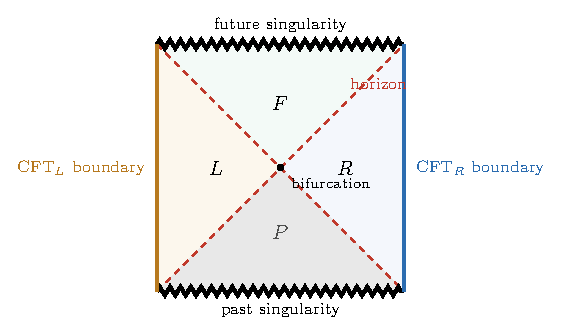
\includegraphics[width=0.72\textwidth]{figs/fig_penrose.pdf}
\caption{Penrose diagram of the two-sided eternal AdS black hole, dual to the thermofield double state $\ket{\Psi_\beta}$. The exterior regions $R$ (blue) and $L$ (gold) end on the AdS boundaries where $\mathrm{CFT}_R$ and $\mathrm{CFT}_L$ live, and are cut off from the interior regions $F$ and $P$ by the event horizons (dashed red), which cross at the bifurcation point (black dot). The wavy lines are the future and past singularities, and the gray horizontal line is the $t=0$ slice, which runs from one boundary to the other through the Einstein--Rosen bridge.}
\label{fig:penrose}
\end{figure}

\subsection*{Two puzzles, and how algebra resolves the first of them}

The $T>T_{\text{HP}}$ phase is identified with an eternal black hole, and this identification passes every
quantitative check. Even so, before the algebraic reformulation it carried two conceptual puzzles. Both are
long-standing and well known in holography.

\textbf{The factorization puzzle.} The boundary theory clearly factorizes as $\text{CFT}_R\otimes
\text{CFT}_L$. It is just two separate, non-interacting copies of the same CFT. But the bulk black hole is a
single, \emph{connected} spacetime. There are bulk operators, such as a Wilson line stretching from the left
boundary through the interior to the right boundary (Fig.~\ref{fig:penrose}), that do not seem to split into an
operator in $B(\HH_R)$ times an operator in $B(\HH_L)$. How can a connected bulk object correspond to anything
in a boundary tensor product that is clearly disconnected?

\textbf{The meeting-behind-the-horizon puzzle.} There is no interaction at all between $\text{CFT}_R$ and
$\text{CFT}_L$: the total Hamiltonian is simply $H_R+H_L$, with no cross term. Yet bulk degrees of freedom that
start separately in the $R$ and $L$ exterior regions can cross the horizon and interact with each other in the
interior. How can two boundary theories that are disconnected, both causally and dynamically, produce bulk
physics that is connected once you look behind the horizon?

The algebraic picture resolves the \emph{first} puzzle directly. Once $N\to\infty$ is taken seriously,
``$B(\HH_R)$'' is the wrong object to compare with the bulk exterior algebra. The actual large-$N$ limit of the
algebra is $Y_R$. It is type $\mathrm{III}_1$, not type I, precisely because of the order-$N^2$ entanglement
between $R$ and $L$. For a type $\mathrm{III}_1$ algebra and its commutant, there is no tensor product structure
$Y_R\otimes Y_L$ inside $B(\HH^{\text{GNS}})$ of the kind an ordinary tensor product would give. So nothing
prevents the presence of operators (such as the boundary counterpart of that Wilson line) that are not products
of an $R$-piece and an $L$-piece. The apparent contradiction came from using type I tensor-product intuition in
a regime where the algebra has already become type $\mathrm{III}_1$.

The second puzzle, meeting behind the horizon, needs more tools. It needs the emergent commutant and the
half-sided modular inclusion structure of Chapter~4. It is taken up in Chapter~8, where the bulk causal
structure of the eternal black hole is built directly from boundary algebra data.

Three further remarks prepare the ground for algebraic ER$=$EPR in Chapter~8.

First, the whole qualitative conclusion here (disconnected bulk geometry below $T_{\text{HP}}$, connected black
hole above it) could in principle have been \emph{deduced} just from watching $Y_R$ jump from type I to type
$\mathrm{III}_1$. No independent knowledge of the bulk geometry is needed.

Second, for $T>T_{\text{HP}}$ different temperatures $\beta$ lie in different, non-overlapping GNS sectors.
Their entanglement entropies differ by an amount of order $N^2$, which is an infinite barrier in the strict
limit (the mechanism of Chapter~1 again). Below $T_{\text{HP}}$, by contrast, every $\beta$ shares one common GNS
Hilbert space, and the different TFD states are just different vectors inside it.

Third, the ordinary Hamiltonians $H_R,H_L$ do not survive the large-$N$ limit as elements of the algebra. So
\eqref{eq:ads-tfd-modular} stops holding literally. But the modular operator $\Delta_\beta$ itself \emph{does}
survive, and it still generates boundary time translation in opposite directions on the two sides. Below
$T_{\text{HP}}$ it splits into an $R$ part and an $L$ part, $-\log\Delta_\beta=\beta(\hat h_R-\hat h_L)$, where
$\hat h$ is the vacuum-sector time-translation operator of the previous section. Above $T_{\text{HP}}$ it does
not split at all. This tracks the transition from type I to type $\mathrm{III}_1$ exactly.

\section{General black holes}

The thermofield double is special. It has an exact bifurcate horizon: the future and past horizons meet at a
single surface in a perfectly symmetric way. A more generic two-sided semiclassical state $\ket\Psi$ is dual to
a ``long'' black hole. Such a black hole has a genuine interior region $I$ that separates $R$ and $L$, and its
horizons do not meet at a single bifurcation surface.

This case shows the subtlety noted at the start of this chapter: the inclusion $\Sscr\subseteq\Alg_\Psi$ can
now be \emph{strict}. The renormalized single-trace algebras still reproduce the bulk exterior algebras,
$Y_R=\widetilde\M_R$ and $Y_L=\widetilde\M_L$. But $R$ and $L$ together no longer cover a full Cauchy slice. The
interior region $I$ is missing. Bulk operators in $I$ must still correspond to \emph{some} boundary operators
that survive the large-$N$ limit, since they belong to the same physical bulk field as the exterior operators,
only evaluated at a different place. But they are not single-trace operators. They must belong to
$\Alg_\Psi\setminus\Sscr$.

Chapter~7 identifies exactly what these extra operators are. They are generated from single-trace operators by
\emph{modular flow}. This mechanism was previewed by the ergodic lemma of Chapter~4: a modular flow, run long
enough, generates a whole larger algebra starting from a smaller subalgebra.

The same phenomenon (extra, non-single-trace operators needed for a black-hole interior) also occurs for a
``long'' one-sided black hole. A one-sided black hole formed by ordinary gravitational collapse, with matter
falling in from empty space, is different. This contrast matters in Chapter~7. There, $\Alg_\Psi=\Sscr$
exactly: single-trace operators are already everything, and nothing extra is needed.

\section{A diagnostic of firewalls in generic highly excited states}

Now consider a completely generic, highly excited state $\ket\Psi$ with energy $E_\Psi\sim O(N^2)$. We do not
assume that it was prepared to have a nice bulk dual. It is just an arbitrary state of that energy. The
boundary theory at such energies is expected to be chaotic. A typical state of that energy should then look
thermal to any probe made of single-trace operators, to leading order in $1/N$:
\begin{equation}
\braket{\Psi|O|\Psi}\approx\braket{O}_\beta, \qquad \braket{\Psi|O_1\cdots O_n|\Psi}\approx\braket{O_1\cdots
O_n}_\beta ,
\label{eq:ads-thermal}
\end{equation}
with $\beta$ fixed by matching the energy, $E_\Psi=E_\beta$. This is the familiar statement, in the spirit of
the eigenstate thermalization hypothesis, that a single generic high-energy state reproduces thermal
correlators. It says that, as far as single-trace operators can tell, $\Psi$ has a smooth black-hole exterior.
But does it also have a smooth \emph{interior}, a genuine continuation of the geometry behind the horizon? Or
does the interior simply fail to exist? The second possibility is called a \textbf{firewall}.

The previous section already gave the criterion needed to answer this. A smooth interior requires operators
that survive the large-$N$ limit \emph{beyond} single-trace operators, that is, $\Sscr\subsetneq\Alg_\Psi$. This
gives a clean, checkable diagnostic. \textbf{Suppose a generic highly excited state satisfies the thermal
condition \eqref{eq:ads-thermal} and \emph{also} has $\Alg_\Psi=\Sscr$, so that no operators beyond single-trace
ones survive the limit. Then its bulk dual has a firewall.} In this case $\omega_\Psi$ is a \emph{mixed} state on
$\Alg_\Psi$. This violates the purity condition \eqref{eq:ads-irreducible} assumed earlier for the ``nice''
semiclassical case.

For two-sided generic states there is an analogous statement with one more condition. The correlations between
the two sides must vanish, $\braket{\Psi|O_RO_L|\Psi}_c\to0$ as $N\to\infty$. This is consistent with there
being no smooth, connected bridge between the two boundaries in that case.

\section{Perturbative \texorpdfstring{$1/N$}{1/N} corrections}

\subsection*{Corrections to bulk reconstruction}

Everything so far worked at strictly leading order in $G_N$, or equivalently in $1/N$. Including subleading
orders makes the bulk field theory interacting: the terms $\kappa S_3+\kappa^2S_4+\cdots$ in the bulk action
switch back on. Correspondingly, the boundary theory develops nonzero connected three-point and higher
functions, suppressed by powers of $1/N$.

One direct consequence is that the HKLL formula \eqref{eq:ads-hkll}, exact at leading order, gets corrected.
Take the simplest case of a cubic self-interaction $\phi^3$ and solve the interacting bulk equation of motion
perturbatively in $\kappa$. (We do not reproduce this computation.) The result is a series of extra terms in the
bulk-to-boundary map:
\[
\begin{split}
\phi(X) ={}& \int d^dx\,K(X;x)\,O^{(0)}(x) \\
&+ \kappa\int d^dx_1\,d^dx_2\,K(X;x_1,x_2)\,O^{(0)}(x_1)O^{(0)}(x_2) + \cdots
\end{split}
\]
The leading-order reconstruction picks up multi-trace corrections, with one extra factor of a single-trace
operator for each order in $1/N$. These corrections underlie the topic of ``$1/N$ corrections to bulk
locality,'' a substantial research area of its own. We do not need to track every term here.

The structural point that matters for everything downstream is this. To any finite order in the $1/N$
expansion, the \emph{type} of each algebra discussed above is expected to stay the same as at leading order.
The heuristic reason is that the spectrum of the modular operator is controlled by its zeroth-order piece. On
this picture, perturbation theory in $1/N$ does not change an algebra's type; only the strict $N\to\infty$ limit
can do that.

\subsection*{Conserved charges, and where gravitational dressing first appears}

The second new feature matters more conceptually, for everything from Chapter~9 onward. Suppose the boundary
CFT has a global $U(1)$ symmetry. Its conserved charge must be rescaled, $\widehat Q\equiv Q/N$, in exactly the
way $\widehat H=H/N$ was, because the current itself scales as $N\Tr(\cdots)$. For a single-trace operator of
unit charge, with the convention $[Q,O(x)]=O(x)$,
\begin{equation}
[\widehat Q,O(x)]=\tfrac1N O(x) .
\label{eq:ads-charge}
\end{equation}
So the action of the rescaled charge is suppressed by $1/N$, exactly as in the time-translation story earlier
in this chapter. Within a given sector there is again a genuine large-$N$ operator $\hat q$ that generates the
full rotation, $[\hat q,O(x)]=O(x)$. Like $\hat h_\Omega$ before it, $\hat q$ cannot be written as the integral of
a local density over a single time slice.

The bulk dual of this boundary global $U(1)$ symmetry is a bulk $U(1)$ \emph{gauge} symmetry. Here something new
and physically important appears once $1/N$ corrections are included. Translate the suppressed commutator
\eqref{eq:ads-charge} to the bulk with the extrapolate dictionary. It forces the bulk gauge field strength and a
charged bulk scalar to have a \emph{nonzero commutator at spacelike separation}. This is an explicit violation of
naive bulk microcausality, order by order in $1/N$.

The violation comes directly from the bulk Gauss-law constraint. The equation of motion
$\nabla_MF^{MN}=\kappa J^N$ ties the electric field on a Cauchy slice to the charges on that same slice, because
Gauss's law is intrinsically nonlocal. The resolution comes back as the central mechanism of Chapter~9. A bulk
charged field $\phi(z,x)$ is not gauge invariant on its own. To build a gauge-invariant operator, one attaches a
\textbf{Wilson line} that runs from the boundary to the point:
\begin{equation}
\Phi(z,x) = e^{-i\kappa V}\phi(z,x), \qquad V=\int_0^z dz'\,A_z(z',x) .
\label{eq:ads-dressed}
\end{equation}
This is a \textbf{dressed observable}. The Wilson line is nonlocal: it depends on the gauge field along a whole
path, not just at one point. This nonlocality produces the nonlocal commutation relations directly, and nothing
mysterious is left over.

\subsection*{Worked calculation: Gauss's law and the dressed operator commutator}

To see this mechanism explicitly in canonical quantization, consider the bulk gauge field
$A_M = (A_t, A_z, A_x)$ on a constant-time Cauchy slice, in the gauge $A_t = 0$. We suppress the factors of the
AdS metric; they do not affect the structure of the argument. The momentum conjugate to $A_z(z,x)$ is the
electric field $E^z(z,x) = F^{zt}(z,x) = \partial_t A_z - \partial_z A_t$. The canonical commutation relation is
\[
\big[A_z(z',x'),\, F^{zt}(z'',x'')\big] = i\,\delta(z'-z'')\,\delta(x'-x'') .
\]
The field $F^{xt}$ is conjugate to $A_x$, so it commutes with $A_z$.

In the quantum theory, Gauss's law is a constraint on physical operators. Define the Gauss operator
\[
G(z'',x'') \equiv \partial_{z''} F^{zt}(z'',x'') + \partial_{x''} F^{xt}(z'',x'') - \kappa\, J^t(z'',x'') .
\]
A physical, gauge-invariant operator must commute with $G$ at every point. Take $\phi(z,x)$ to create one unit
of charge at $(z,x)$, so that $[J^t(z'',x''),\phi(z,x)]=\delta(z''-z)\,\delta(x''-x)\,\phi(z,x)$.

The naive, undressed field fails this test. It commutes with the gauge field, $[\phi(z,x), F^{Mt}] = 0$, so only
the charge term contributes:
$[G(z'',x''),\phi(z,x)]=-\kappa\,\delta(z''-z)\,\delta(x''-x)\,\phi(z,x)\ne0$. So $\phi$ is not gauge invariant.

Now compute with the dressed operator $\Phi(z,x) = e^{-i\kappa V(z,x)}\phi(z,x)$, where
$V(z,x) = \int_0^z dz' A_z(z',x)$. First, the commutator with the electric field:
\begin{align}
\big[\Phi(z,x),\, F^{zt}(z'',x'')\big]
&\eqstep{1} \Big[e^{-i\kappa \int_0^z dz' A_z(z',x)},\, F^{zt}(z'',x'')\Big]\,\phi(z,x) \notag\\
&\eqstep{2} -i\kappa \left(\int_0^z dz' \big[A_z(z',x),\, F^{zt}(z'',x'')\big]\right) \Phi(z,x) \notag\\
&\eqstep{3} -i\kappa \left(\int_0^z dz' \, i\,\delta(z'-z'')\,\delta(x-x'')\right) \Phi(z,x) \notag\\
&\eqstep{4} \kappa\,\theta(z - z'')\,\delta(x - x'')\,\Phi(z,x) . \notag
\end{align}
\stepwhy{1}{move $\phi(z,x)$ out of the commutator. It commutes with $F^{zt}$, so only the Wilson-line factor
has to be commuted.}\quad
\stepwhy{2}{$[V,F^{zt}]$ is a $c$-number, so $[e^{-i\kappa V},F^{zt}]=-i\kappa[V,F^{zt}]\,e^{-i\kappa V}$
exactly. Then recombine $e^{-i\kappa V}\phi=\Phi$.}\quad
\stepwhy{3}{substitute the canonical commutator $[A_z(z',x),F^{zt}(z'',x'')]=i\delta(z'-z'')\delta(x-x'')$.}\quad
\stepwhy{4}{$(-i)(i)=1$. The $\delta(z'-z'')$ collapses the $z'$ integral. The result is $1$ if $0<z''<z$ and $0$
if $z''>z$, which is the step function $\theta(z-z'')$.}

Next, differentiate with respect to $z''$:
\begin{align}
\partial_{z''} \big[\Phi(z,x),\, F^{zt}(z'',x'')\big]
&\eqstep{5} \kappa\, \frac{d}{dz''}\theta(z - z'')\;\delta(x - x'')\,\Phi(z,x) \notag\\
&\eqstep{6} -\kappa\,\delta(z'' - z)\,\delta(x'' - x)\,\Phi(z,x) . \notag
\end{align}
\stepwhy{5}{differentiate the result of step (4). Only the step function depends on $z''$.}\quad
\stepwhy{6}{$\frac{d}{dz''}\theta(z-z'')=-\delta(z''-z)$, the derivative of a step function.}

Finally, assemble the Gauss operator:
\begin{align}
[G(z'',x''),\Phi(z,x)]
&\eqstep{7} -\partial_{z''}\big[\Phi(z,x),F^{zt}(z'',x'')\big] - \kappa\big[J^t(z'',x''),\Phi(z,x)\big] \notag\\
&\eqstep{8} \kappa\,\delta(z''-z)\,\delta(x''-x)\,\Phi(z,x) \notag\\
&\qquad - \kappa\,\delta(z''-z)\,\delta(x''-x)\,\Phi(z,x) \ =\ 0 . \notag
\end{align}
\stepwhy{7}{$[\partial F,\Phi]=-\partial[\Phi,F]$. The $F^{xt}$ term drops out because $\Phi$ contains only
$A_z$ and $\phi$, both of which commute with $F^{xt}$.}\quad
\stepwhy{8}{use step (6) for the first term. For the second, $J^t$ commutes with the gauge field, so
$[J^t,\Phi]=e^{-i\kappa V}[J^t,\phi]=\delta\,\Phi$.}

So Gauss's law holds identically as an operator statement for the dressed field. The price is visible in step
(4). For every point $z''<z$ along the string that runs from the boundary to the insertion point, the
commutator with the electric field is nonzero, even though that point is spacelike-separated from $(z,x)$. The
nonlocal string of the Wilson line is the physical cost of gauge invariance.

The same story holds for spacetime symmetries in place of an internal $U(1)$. To make a bulk operator
diffeomorphism-invariant, one must dress it to the boundary with a \emph{gravitational} Wilson line.
Equivalently, one can work in a specific gauge and solve the constraint directly, as in the Gauss-law
calculation above. This dressing produces an analogous $1/N$ correction to the rescaled Hamiltonian,
$\widehat H=\widehat H^{(0)}+\tfrac1N\hat h_\Omega+\cdots$. \textbf{This is the first appearance, in perturbation
theory, of the mechanism that Chapter~9 turns into an exact, nonperturbative construction.} Dressing an operator
gravitationally to a physical reference is what makes it a genuine, gauge-invariant, physical observable. Here
the reference is a Wilson line; in Chapter~9 it is an observer's own clock, through the crossed product of
Chapter~5. The dressing is not optional decoration. It is forced by the bulk Gauss-law constraint that any
theory with gravity or gauge fields must satisfy.

\bigskip
\noindent The large-$N$ algebraic structure of AdS/CFT is now in place: semiclassical states as GNS sectors,
single-trace algebras $Y_O$, a change of algebra type that tracks the Hawking--Page transition, and
gravitational dressing already visible in perturbation theory. Chapter~7 assembles all of this into the central
physical claim of these notes, \textbf{subregion-subalgebra duality}. This is the statement that a bulk causal
region is identical, not merely related, to a specific emergent boundary operator subalgebra.
